\documentclass[11pt,a4paper]{article}
\usepackage[margin=1in]{geometry}
\usepackage{graphicx}
\usepackage{xcolor}
\usepackage{titlesec}
\usepackage{enumitem}
\usepackage{fancyhdr}
\usepackage{booktabs}
\usepackage{longtable}
\usepackage{hyperref}
\usepackage{tcolorbox}
\tcbuselibrary{skins}

\definecolor{primaryblue}{RGB}{45,85,160}
\definecolor{lightgray}{RGB}{245,245,245}

\titleformat{\section}{\large\bfseries\color{primaryblue}}{\thesection}{1em}{}
\titleformat{\subsection}{\normalsize\bfseries\color{primaryblue}}{\thesubsection}{1em}{}

\pagestyle{fancy}
\fancyhf{}
\fancyhead[L]{Thapar Auto --- Prototype Document}
\fancyhead[R]{\thepage}
\renewcommand{\headrulewidth}{0.3pt}

\newtcolorbox{screenbox}[1]{
  colback=lightgray, colframe=primaryblue, fonttitle=\bfseries,
  title=#1, boxrule=0.6pt, arc=2pt
}

\title{\textbf{\Large Thapar Auto} \\[4pt] \large Prototype Document}
\author{Product \& System Design Prototype \\ Thapar Institute of Engineering and Technology}
\date{\today}

\begin{document}
\maketitle
\thispagestyle{fancy}

\section{Overview}
\textbf{Thapar Auto} is a shared campus auto-rickshaw booking and pooling application
built for Thapar Institute of Engineering and Technology. It allows students to book
seats on autos plying between campus stops, with the system automatically pooling
compatible requests onto autos already en route, or dispatching the next idle auto
from a queue when no match exists. Drivers register their vehicle and UPI QR code,
join an idle queue, and receive trip assignments through the app.

\textbf{Technology stack:}
\begin{itemize}[leftmargin=*, itemsep=2pt]
  \item \textbf{Frontend:} Flutter (Android, iOS, Web, Windows, Linux targets)
  \item \textbf{Backend:} Node.js + Express REST API
  \item \textbf{Database:} SQLite (via \texttt{better-sqlite3})
  \item \textbf{Auth:} Google Sign-In restricted to \texttt{@thapar.edu} accounts (students);
        Firebase Phone-OTP authentication (drivers)
  \item \textbf{Payments:} UPI QR code scan-and-pay (driver-supplied static QR)
\end{itemize}

\section{Prototype Scope}
This prototype implements the end-to-end booking loop: role selection $\rightarrow$
authentication $\rightarrow$ stop/seat selection $\rightarrow$ live availability
$\rightarrow$ booking request $\rightarrow$ UPI payment $\rightarrow$ trip confirmation,
alongside the symmetric driver flow: registration $\rightarrow$ idle queue
$\rightarrow$ dispatch/pooling $\rightarrow$ trip completion. Live GPS tracking of the
auto is explicitly out of scope for this iteration.

\section{Screen-by-Screen Walkthrough}

\begin{screenbox}{Screen 1 --- Role Selection}
\textbf{Route:} \texttt{RoleSelectScreen} (app entry point) \\[4pt]
\textbf{Purpose:} Lets the user declare whether they are a Student or a Driver before
any authentication happens. \\[4pt]
\textbf{Key elements:}
\begin{itemize}[leftmargin=*, itemsep=1pt]
  \item App icon (\emph{directions\_car\_filled}) and title \textit{``Thapar Auto''}
        with tagline \textit{``Campus auto booking, made fast.''}
  \item Primary button \textbf{``I'm a Student''} $\rightarrow$ navigates to the
        Student Login screen
  \item Secondary (outlined) button \textbf{``I'm a Driver''} $\rightarrow$ navigates
        to the Driver Login screen
\end{itemize}
\end{screenbox}

\begin{screenbox}{Screen 2 --- Student Login}
\textbf{Route:} \texttt{StudentLoginScreen} \\[4pt]
\textbf{Purpose:} Authenticates the student via Google Sign-In and restricts access to
institute email addresses. \\[4pt]
\textbf{Flow:}
\begin{enumerate}[leftmargin=*, itemsep=1pt]
  \item Student taps \textbf{Sign in with Google}.
  \item The returned account email is checked against the \texttt{@thapar.edu} domain;
        non-institute accounts are signed out immediately with an inline error.
  \item On success, the app calls \texttt{POST /students} to register/fetch the
        student record, then stores the session in \texttt{AppState} and navigates to
        the Student Home screen.
\end{enumerate}
\textbf{Note:} the current prototype trusts the client-supplied email; production
would additionally verify the Google ID token server-side.
\end{screenbox}

\begin{screenbox}{Screen 3 --- Student Home (Booking)}
\textbf{Route:} \texttt{StudentHomeScreen} \\[4pt]
\textbf{Purpose:} Core booking screen --- the student selects pickup/drop stops and
seat count, watches live pooling availability, and submits a booking request. \\[4pt]
\textbf{Key elements:}
\begin{itemize}[leftmargin=*, itemsep=1pt]
  \item \textbf{Pickup} and \textbf{Drop} location dropdowns (\texttt{LocationDropdown}),
        populated from \texttt{GET /locations}
  \item \textbf{Seat selector} widget (1--capacity)
  \item Live \textbf{availability panel} --- debounced call to
        \texttt{GET /availability} on every selection change, showing poolable
        enroute autos and idle-queue count
  \item \textbf{Request Booking} primary button $\rightarrow$ \texttt{POST /bookings}
\end{itemize}
\end{screenbox}

\begin{screenbox}{Screen 4 --- Payment}
\textbf{Route:} \texttt{StudentPaymentScreen} \\[4pt]
\textbf{Purpose:} Displays the assigned driver's UPI QR code and fare so the student
can pay before boarding. \\[4pt]
\textbf{Flow:}
\begin{enumerate}[leftmargin=*, itemsep=1pt]
  \item On load, fetches the assigned auto (\texttt{GET /autos/:id}) and its driver
        (\texttt{GET /drivers/:id}) to display the QR image and driver details.
  \item Student scans the QR and pays externally, then taps \textbf{I've Paid}.
  \item App calls \texttt{POST /bookings/:id/pay}, flipping the booking's
        \texttt{payment\_status} to \texttt{PAID}.
  \item Navigates to the Trip Status screen.
\end{enumerate}
\textbf{Note:} this is a scan-and-confirm flow, not a verified payment gateway
webhook --- flagged in-code for production hardening.
\end{screenbox}

\begin{screenbox}{Screen 5 --- Trip Status (Confirmation)}
\textbf{Route:} \texttt{StudentTripStatusScreen} \\[4pt]
\textbf{Purpose:} Confirms the booking and summarizes the trip. \\[4pt]
\textbf{Key elements:}
\begin{itemize}[leftmargin=*, itemsep=1pt]
  \item Success icon and \textit{``You're booked!''} message
  \item Contextual message distinguishing a \textbf{pooled} booking (joined an
        already-enroute auto) from a \textbf{freshly dispatched} one
  \item Trip summary card: pickup $\rightarrow$ drop, seats booked, fare paid,
        truncated booking ID
  \item \textbf{Book Another Ride} button, returning to Student Home
\end{itemize}
\end{screenbox}

\begin{screenbox}{Screen 6 --- Driver Login \& Registration}
\textbf{Route:} \texttt{DriverLoginScreen} \\[4pt]
\textbf{Purpose:} Three-step driver onboarding: phone verification, then vehicle
details. \\[4pt]
\textbf{Steps (\texttt{\_Step} enum):}
\begin{enumerate}[leftmargin=*, itemsep=1pt]
  \item \textbf{Phone} --- driver enters mobile number; Firebase sends an OTP.
  \item \textbf{OTP} --- 6-digit code entry with a 59-second countdown and resend.
  \item \textbf{Details} --- name, vehicle number, capacity (4/5/7-seater selector),
        and a required UPI QR code image upload (via \texttt{image\_picker}).
\end{enumerate}
On submission, calls \texttt{POST /drivers} (multipart, with the QR image), which
also creates the driver's \texttt{auto} record and places it at the back of the idle
queue.
\end{screenbox}

\begin{screenbox}{Screen 7 --- Driver Dashboard}
\textbf{Route:} \texttt{DriverDashboardScreen} \\[4pt]
\textbf{Purpose:} Live operating screen for a driver once registered; polls the
backend every 5 seconds. \\[4pt]
\textbf{States shown:}
\begin{itemize}[leftmargin=*, itemsep=1pt]
  \item \textbf{Idle:} current position in the idle queue
        (\texttt{GET /autos/:id/queue-position})
  \item \textbf{Enroute:} list of current trip's bookings
        (\texttt{GET /autos/:id/bookings}), including student name, pickup/drop,
        seats and payment status
  \item \textbf{Mark Trip Complete} button $\rightarrow$
        \texttt{POST /autos/:id/complete-trip}, which resets the auto to idle and
        re-queues it at the back
\end{itemize}
\end{screenbox}

\section{Navigation Map}
\begin{center}
\begin{tabular}{ll}
\toprule
\textbf{From} & \textbf{To} \\
\midrule
Role Select & Student Login / Driver Login \\
Student Login & Student Home (on successful auth) \\
Student Home & Payment (on successful booking request) \\
Payment & Trip Status (on payment confirmation) \\
Trip Status & Student Home (Book Another Ride) \\
Driver Login & Driver Dashboard (on successful registration) \\
Driver Dashboard & (self-refreshing; no forward navigation) \\
\bottomrule
\end{tabular}
\end{center}

\section{System Design References}
The following diagrams accompany this prototype and are included in the delivered
package:
\begin{itemize}[leftmargin=*, itemsep=2pt]
  \item \textbf{Use-Case Diagram} and \textbf{Data Flow Diagrams (Levels 0--2)} ---
        see \texttt{Thapar\_Auto\_System\_Design\_Diagrams.md}
  \item \textbf{Entity-Relationship Diagram} --- \texttt{er\_diagram.png}
        (Figure~\ref{fig:er})
  \item \textbf{Activity Diagram} (booking \& dispatch flow) ---
        \texttt{activity\_diagram.jpg} (Figure~\ref{fig:activity})
  \item \textbf{Project Gantt Chart} --- \texttt{gantt\_chart.pdf}
\end{itemize}

\begin{figure}[h!]
  \centering
  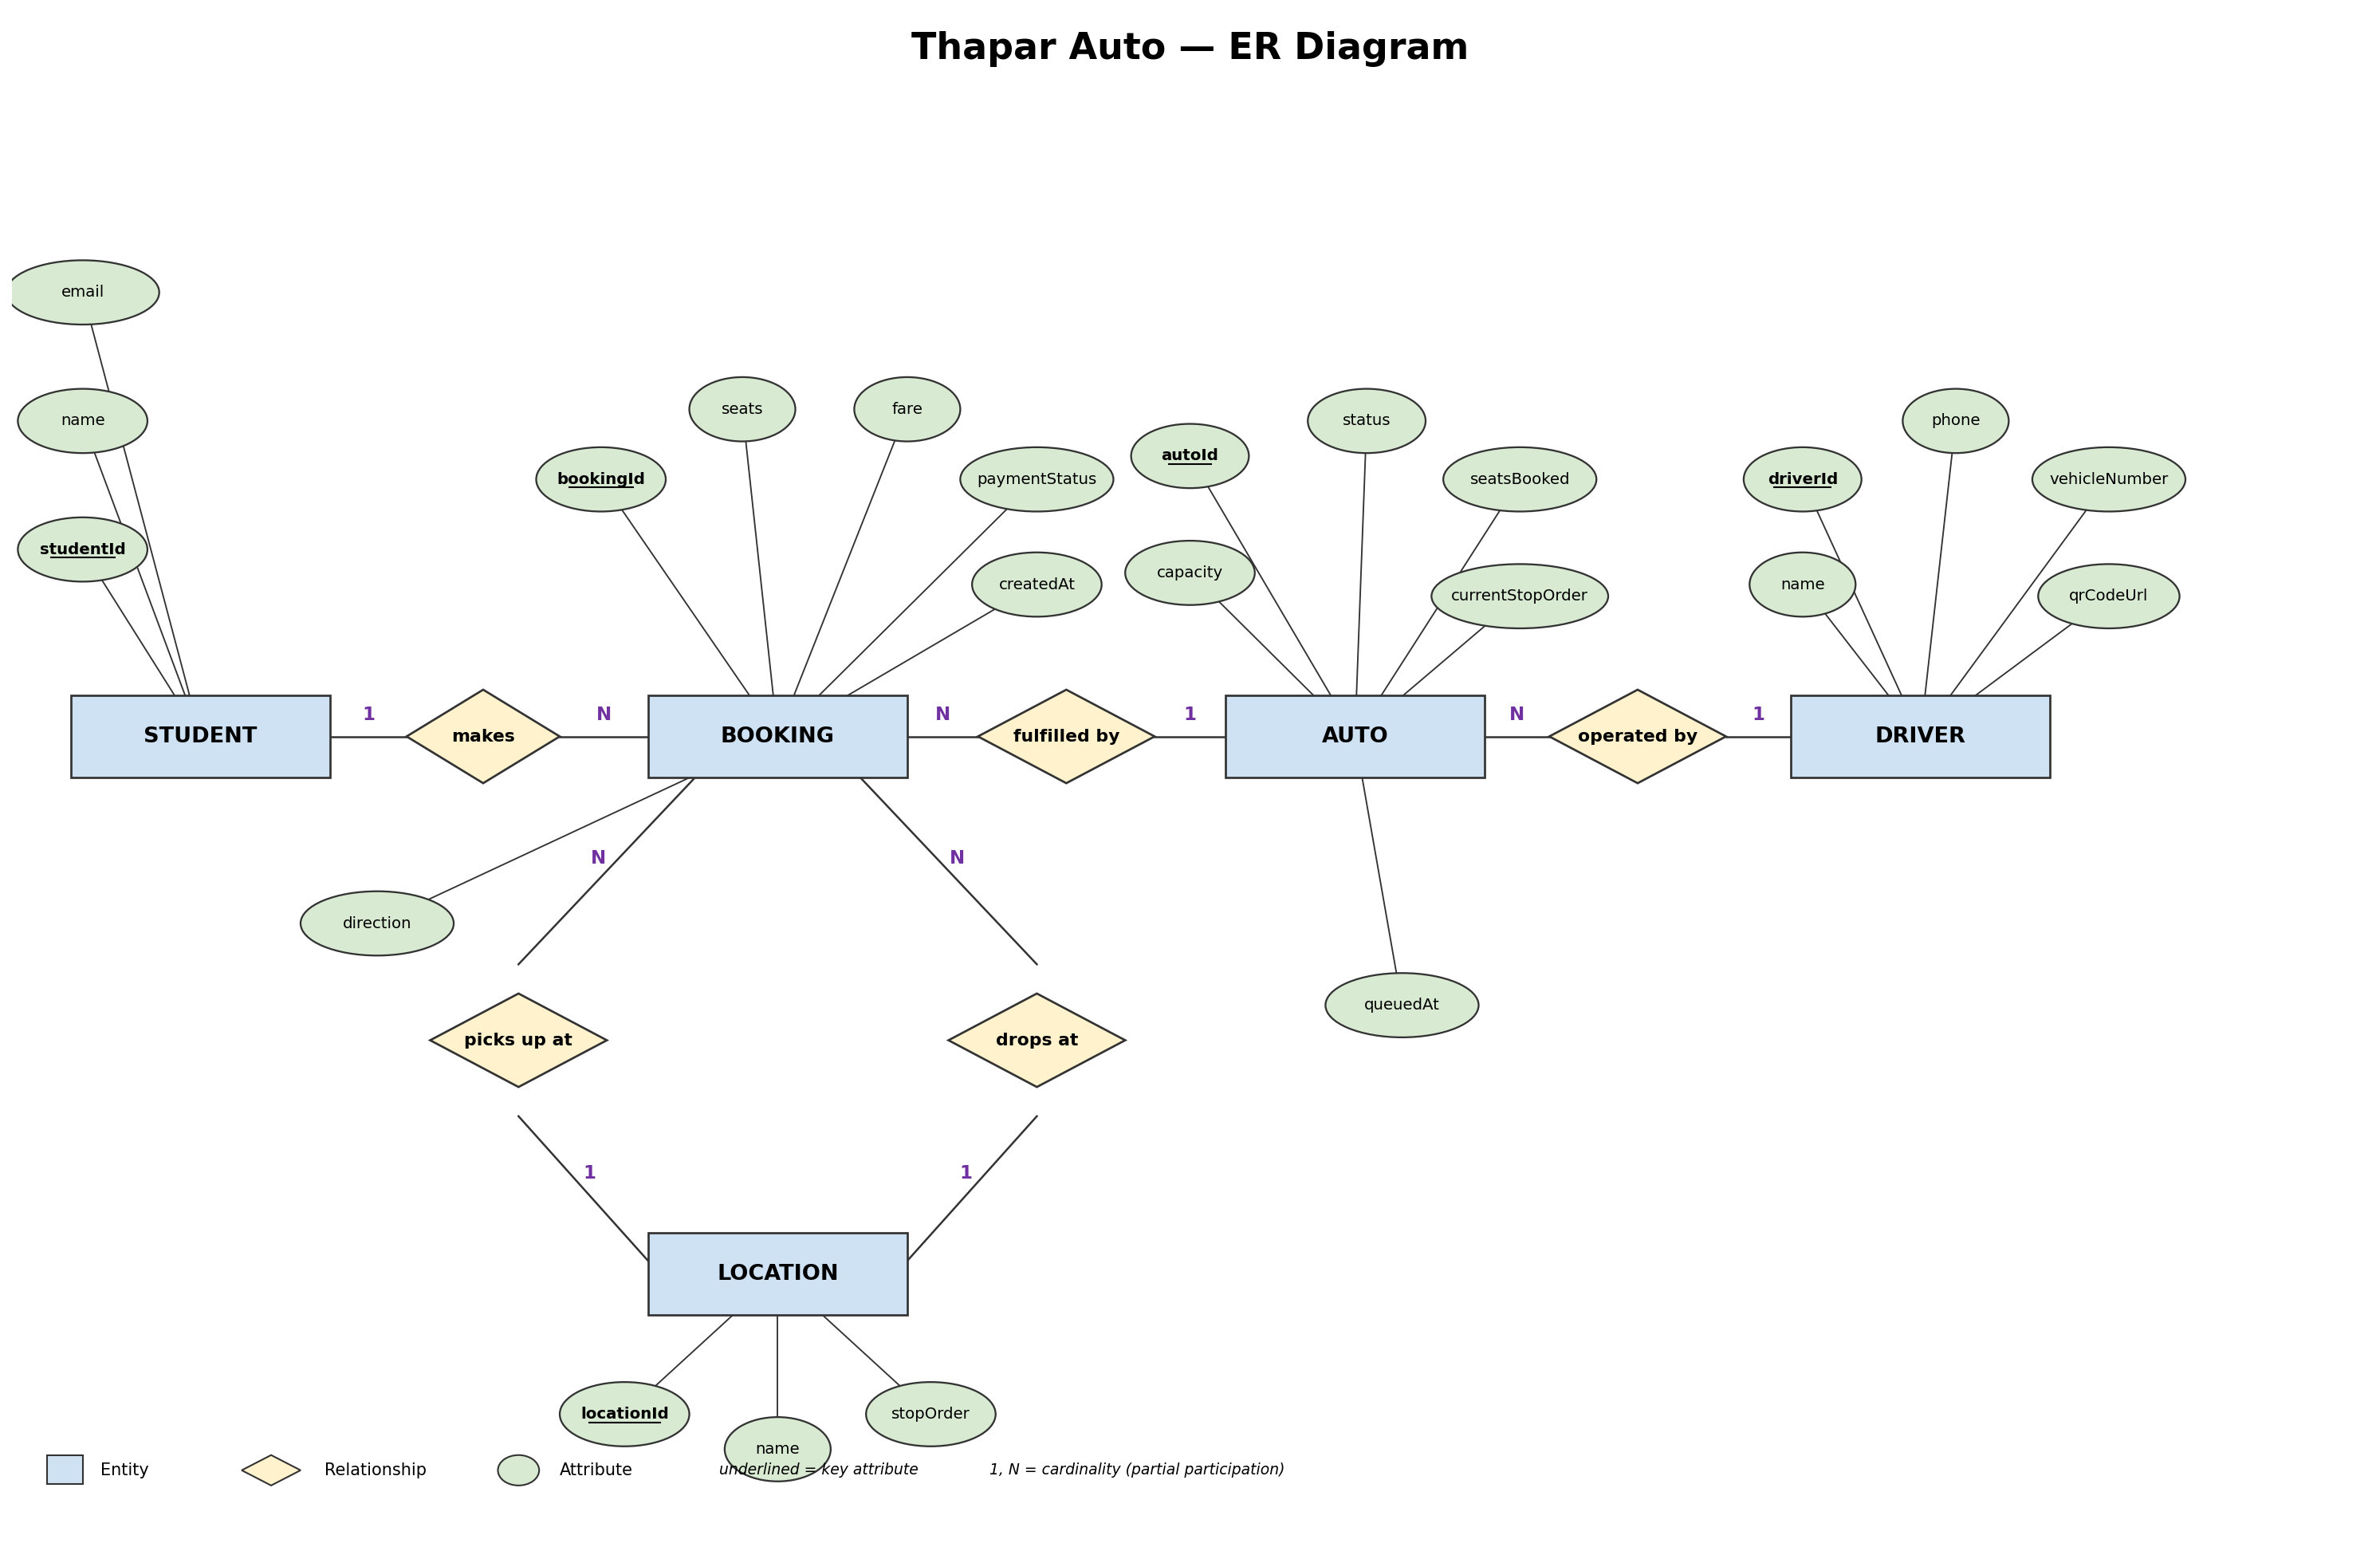
\includegraphics[width=\textwidth]{er_diagram.png}
  \caption{Entity-Relationship Diagram --- Thapar Auto}
  \label{fig:er}
\end{figure}

\begin{figure}[p]
  \centering
  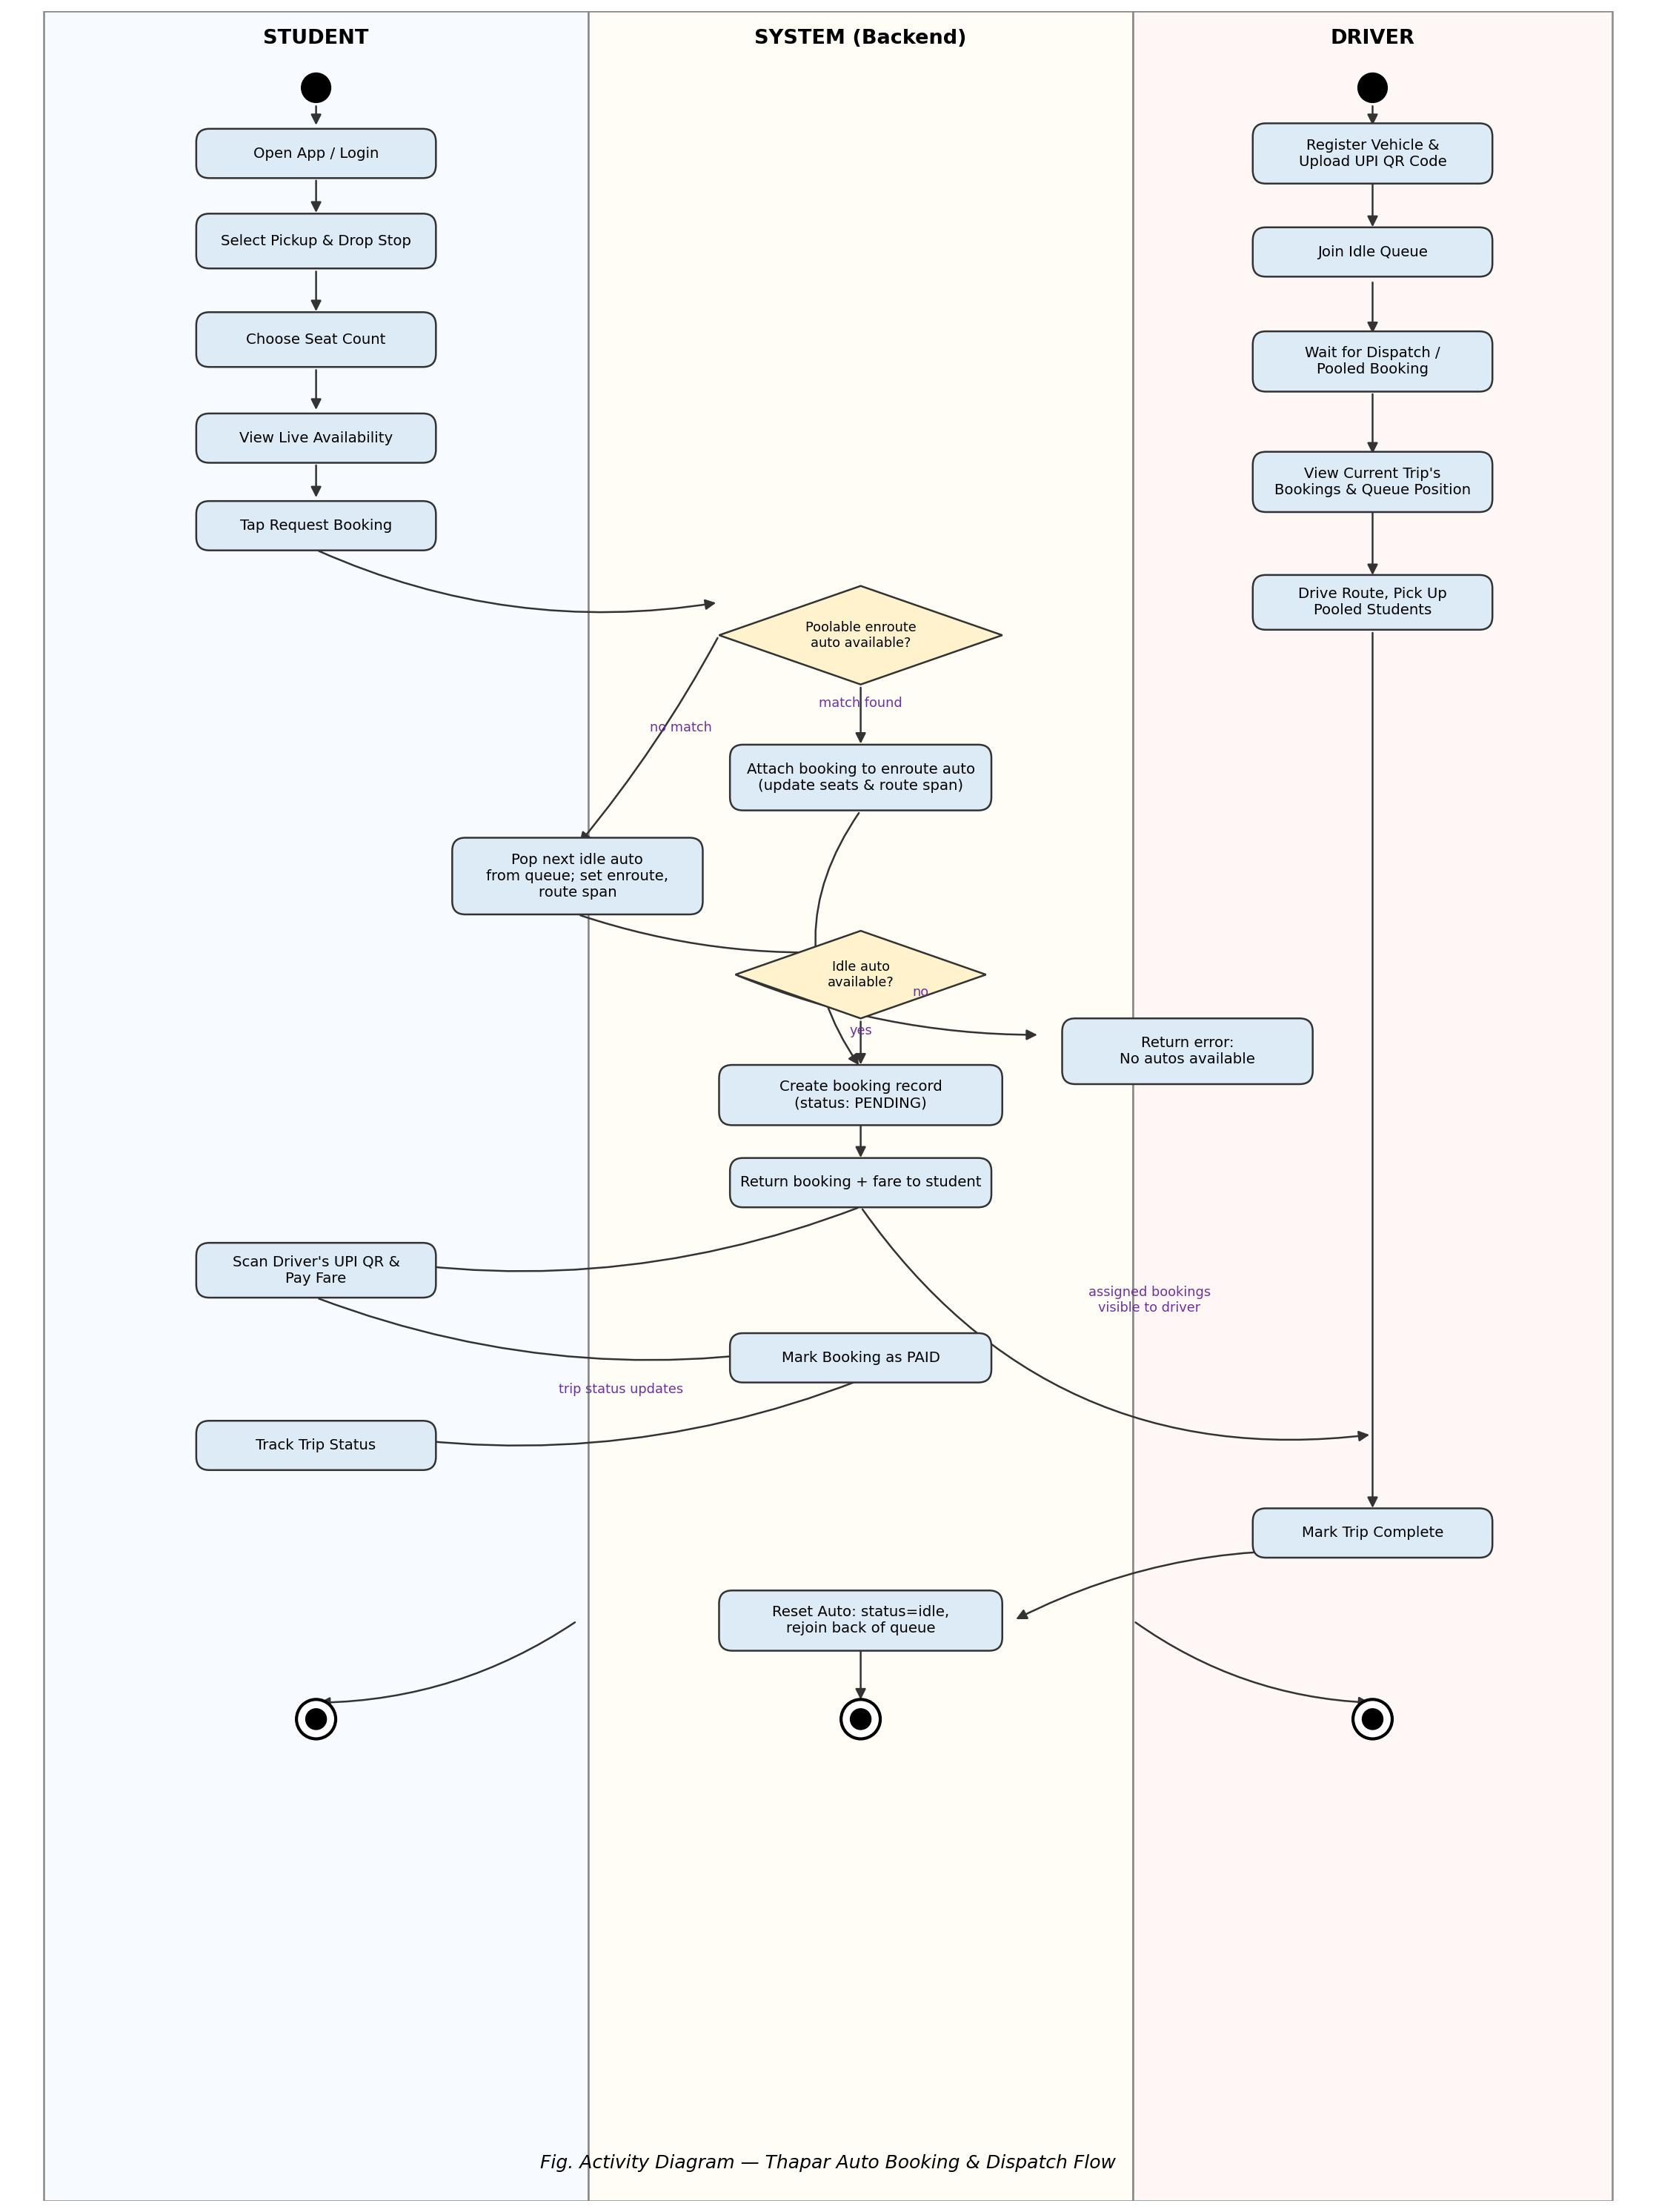
\includegraphics[width=0.85\textwidth]{activity_diagram.jpg}
  \caption{Activity Diagram --- Booking \& Dispatch Flow}
  \label{fig:activity}
\end{figure}

\section{Data Model Summary}
\begin{center}
\begin{longtable}{p{2.7cm}p{9.5cm}}
\toprule
\textbf{Table} & \textbf{Purpose} \\
\midrule
\texttt{locations} & Ordered campus stops (\texttt{stop\_order} drives routing/direction logic) \\
\texttt{students} & Student profile, restricted to \texttt{@thapar.edu} \\
\texttt{drivers} & Driver profile, vehicle capacity, UPI QR image URL \\
\texttt{autos} & One per driver; tracks \texttt{status} (idle/enroute), \texttt{seats\_booked}, direction and route span, and idle-queue timestamp \\
\texttt{bookings} & Student's seat request: pickup/drop, seats, fare, \texttt{payment\_status} \\
\bottomrule
\end{longtable}
\end{center}

\section{Matching Logic (Summary)}
On a booking request, the backend first searches for an \textbf{enroute} auto heading
the same direction whose remaining capacity and route span can absorb the new
pickup/drop (pooling). If none qualifies, the \textbf{next idle auto} is popped from
the FIFO queue and dispatched fresh. Completed trips return the auto to the back of
the idle queue. Fare is a flat \textbf{Rs.\ 10 per seat}.

\end{document}
